\section{Filtering Monitoring Events}
\label{sec:filter}

The instruction-grained monitoring techniques we consider forward all
instructions of certain types (e.g., load instructions) to the monitoring core.
However, not all of these forwarded instructions have relevant monitoring to be
done. For example, for array bounds check, all load and store instructions are
forwarded. However, only loads and stores associated with array pointers have
relevant monitoring operations to be done. Thus, we can greatly reduce the amount of
monitoring done by only forwarding instructions to the monitoring core that 
correspond to array pointers. These accesses can be identified because their
corresponding metadata has been set with base and bound information.
More generally, we can reduce monitoring overheads by filtering out 
events that correspond to clean or uninitialized metadata.

% Overview of inserting dataflow engine
\begin{figure}
  \begin{center}
    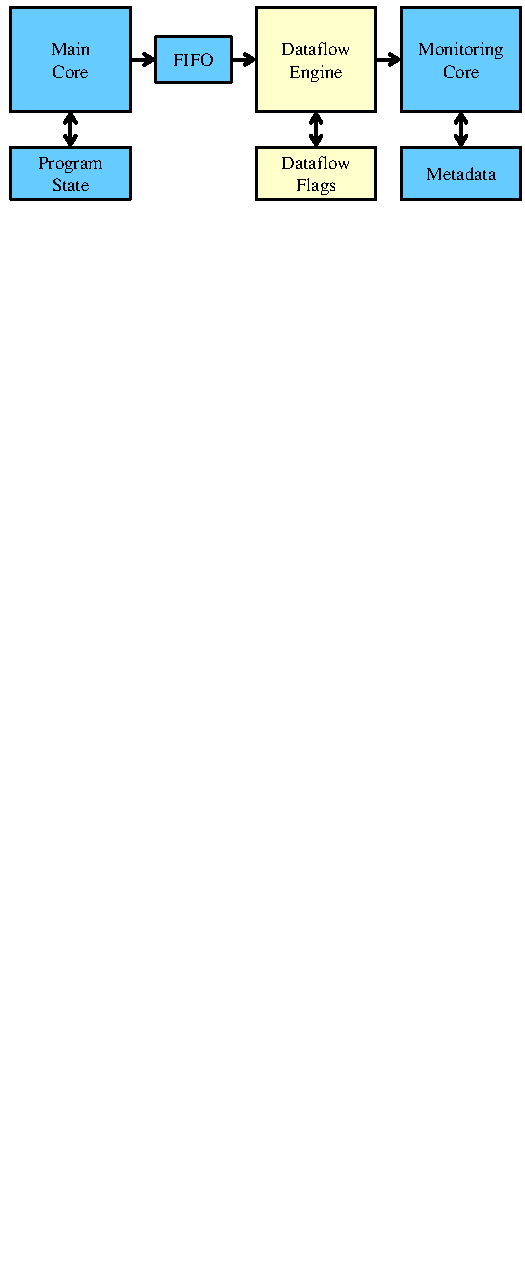
\includegraphics[width=\columnwidth]{figs/dataflow_overview.pdf}
    \vspace{-0.2in}
    \caption{The dataflow engine is inserted between the main core and the monitoring core.}
    \label{fig:filter.overview} 
    \vspace{-0.1in}
  \end{center}
\end{figure}

In this section, we describe how we can use a dataflow tracking engine to
efficiently track clean metadata. This engine sits between the main core and
the monitoring core (see Figure~\ref{fig:filter.overview}) in order to filter
out monitoring operations for clean metadata.

\subsection{Tracking Clean Metadata}

% Detailed architecture of dataflow engine
\begin{figure*}
  \begin{center}
    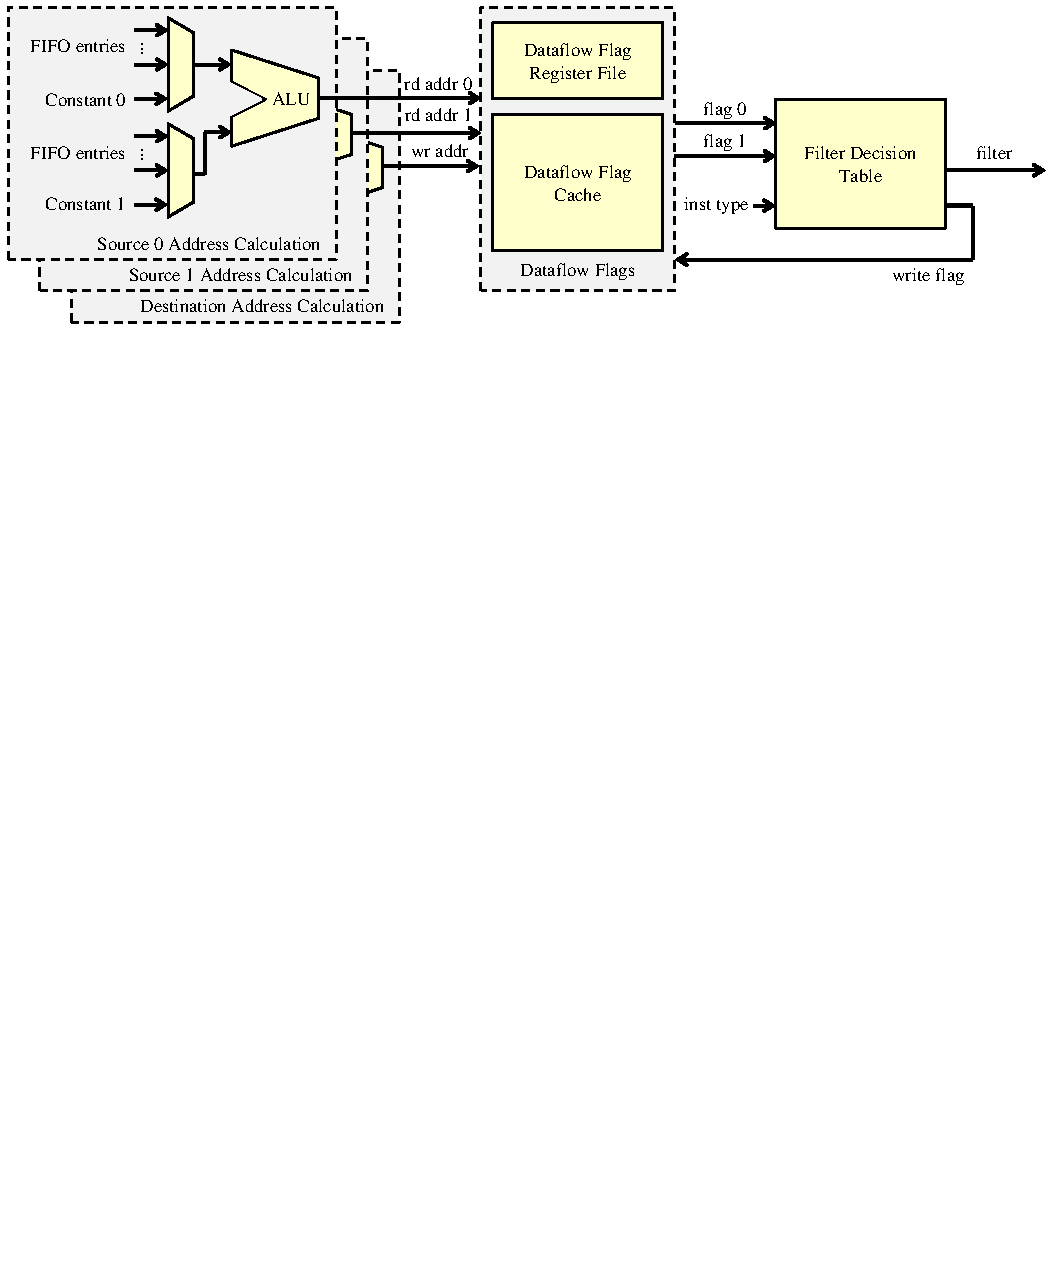
\includegraphics[width=\linewidth]{figs/dataflow_architecture.pdf}
    \vspace{-0.3in}
    \caption{Hardware architecture for dataflow engine.}
    \label{fig:filter.architecture} 
    \vspace{-0.1in}
  \end{center}
\end{figure*}

Figure~\ref{fig:filter.architecture} shows a block diagram of the dataflow
tracking engine for
keeping track of clean metadata. Initially, all metadata is marked as clean.
When the monitoring core writes a non-null metadata value, it also sends a
signal to the dataflow engine to mark the metadata as dirty. 

When a monitoring event arrives at the dataflow engine,
it reads in up to two clean flags. A table is used to configure
which clean flags should be read in depending on the instruction type of
the event and information from the monitoring event. A pair of simple ALUs are
used to allow calculating memory addresses based on information from the
monitoring event. Typically, the clean flags read correspond to the
source operands of the monitored instruction.

Given this set of clean flags, a Filter Decision Table decides, based
on instruction type, whether an event can be filtered out. This table is
configured based on the specific semantics of a monitoring technique.
Typically, if all clean flags are marked as clean, then the
event can be filtered out. For example, for array bounds check, if the source
register's metadata is marked as clean, then this means that the
register does not correspond to an array pointer. Thus, we can filter out the
monitoring operation for this event. 
It is important that we also propagate the clean information to the destination
of the instruction.  The Filter Decision Table also includes a bit indicating
whether the destination operand metadata should be marked as uninitialized.
